\chapter{Monero} \label{sec:Monero}
%
\epigraph{They who can give up essential liberty to obtain a little temporary safety deserve neither liberty nor safety.}{\textit{Benjamin Franklin}}
%
\section{Introduction}
Monero (XMR) is a decentralised open-source cryptocurrency. The project's fundamental feature is privacy - it aims to be a digital medium of exchange with untraceable payments, unlinkable transactions and resistance to blockchain analysis. The parties behind a Monero transaction are not known; this results in considerable increase of privacy compared to Bitcoin and its forks~\cite{monero}.

\section{History}
First, the construction was outlined in an October 2013 white paper by the pseudonymous figure Nicolas van Saberhagen and called \hyperref[sec:CryptoNote]{CryptoNote}  protocol~\cite{citeulike:14139412}. Later, in 2014, Bitcointalk forum user known as \verb|thankful_for_today| forked the codebase of \emph{Bytecoin} (CryptoNote's reference implementation) into the name \emph{BitMonero}, which is a compound of bit and monero (literally meaning \emph{coin} in Esperanto~\cite{esperanto}).

The release of BitMonero was very poorly received by the community that initially backed it. Plans to fix and improve Bytecoin with changes to block time, tail emission and block reward had all been ignored, and \verb|thankful_for_today| simply disappeared from the development scene. A group of users led by \verb|Johnny Mnemonic|\footnote{Fun fact: reference to a 90's cult film character, incarnated by Keanu Reeves, who could store data into his mind and worked as a data courier.} decided that the community should take over the project and five days later they did, while also changing the name to \emph{Monero}.
\pagebreak

Due to its privacy features, Monero experienced rapid growth in market capitalization and transaction volume during the year 2016, faster and bigger than any other cryptocurrency that year. This growth was driven by its uptake in the darknet market. From the beginning, Monero has been used by people holding other cryptocurrencies like \hyperref[sec:Bitcoin]{Bitcoin} to break the link between transactions, with the other cryptocoins first converted to Monero, then after some delay converted back and sent to an address unrelated to those used before.

On January 10, 2017, the privacy of Monero transactions was further strengthened by the adoption of Bitcoin Core developer Gregory Maxwell's algorithm \emph{Confidential Transactions}~\cite{ringCT}, hiding the amounts being transacted, in combination with an improved version of \emph{Ring Signatures}.

%\setlength{\intextsep}{0pt}
\begin{wrapfigure}[4]{R}{0.3\textwidth}
\centering

\includegraphics[width=0.3\textwidth]{Images/Monero/coinhive.jpg}
\end{wrapfigure}
In late 2017, malware and antivirus service providers blocked a JavaScript implementation of Monero miner \emph{Coinhive}~\cite{coinhive} that was embedded in websites and apps. Coinhive generated the script as an alternative to advertisements; a website or app could embed it and use website visitor's CPU to mine the cryptocurrency, while the visitor was consuming the content of the webpage.

However, some websites and apps did this without informing visitors and some hackers implemented it in a way that drained visitors' CPUs. As a result, the script was blocked by companies that offer ad blocking subscription lists, antivirus services and antimalware services.

Monero is actively encouraged to those seeking financial privacy, since payments and account balances remain entirely hidden, which is not the standard for most cryptocurrencies.

\section{Specifications}
Monero is~\cite{monero}:
\begin{description}
  \item [Untraceable] Monero uses a digital signature scheme called \emph{ring signatures}~\cite{ringCT}, which shuffles users' public keys in order to eliminate the possibility to identify a particular user.
  \item [Unlinkable] Monero employs a specific protocol which generates multiple unique one-time addresses that can only be linked by the payment receiver and are unfeasable to be revealed through blockhain analysis.
  \item [Secure] Monero is cryptographically secured. Moreover, the design of the algorithm used consists in tremendous computational and electric capabilities, that an adversary would need to even try to steal funds.
  \item [Private] Privacy is basically provided by the idea of anonymous transactions without any obligations to cooperate with third parties.
  \item [Analysis Resistant] Monero's blockchain analysis resistance results from unlinkability, which is achieved by using a modified version of the Diffie-Hellman exchange protocol~\cite{Diffie:2006:NDC:2263321.2269104} that generates multiple one-time public addresses that can only be simply gathered by the message receiver, but hardly analyzed by confused foreigners inside the block explorer.
\end{description}
\pagebreak

\subsection{Account}
%\setlength{\intextsep}{0pt}
\begin{wrapfigure}[5]{L}{0.3\textwidth}
\centering
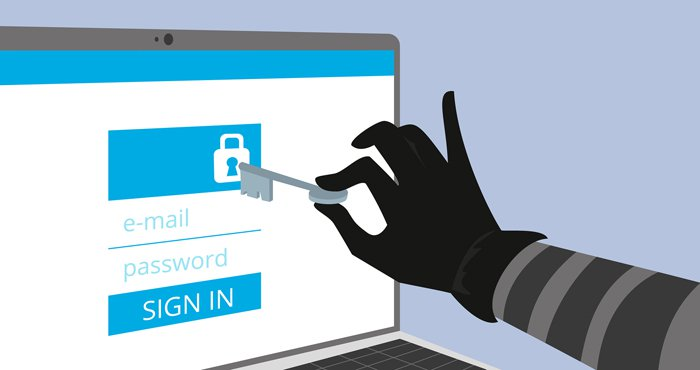
\includegraphics[width=0.3\textwidth]{Images/Monero/account.jpg}
\end{wrapfigure}
In Monero, a wallet is called an account and it is a private account owned and operated by a Monero user. An account contains all of the Monero transactions a user has sent and received. Some user's account balance is a sum of all the Monero received, less the Monero sent.

A Monero account has two balances, a locked and an unlocked balance. The unlocked balance contains funds that can be spent immediately, and the locked balance contains funds that can't be spent right away. A Monero user may receive a transaction that has an unlock time set or he/she may have sent some Monero and is waiting for the change to come back to his/her wallet, both of which situations could lead to those funds being locked for a time.

An account resides only under user's control, normally on his/her computer, and cannot be accessed by anyone else if he/she practices good security~\cite{getmonero}.

\subsection{Keys}
%\setlength{\intextsep}{0pt}
\begin{wrapfigure}[5]{L}{0.2\textwidth}
\centering
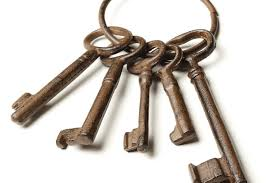
\includegraphics[width=0.2\textwidth]{Images/Monero/keys.jpg}
\end{wrapfigure}
A Monero account is based on two keys. They are called \emph{spend key} and \emph{view key}. The \emph{spend key} is special in that it is the single key required to spend your Monero funds, whereas the \emph{view key} allows you to reveal your transactions to a third party. That makes sense in case of auditing or accounting purposes.
\vspace{0.8cm}

The spine of the Monero project is the \hyperref[sec:CryptoNote]{CryptoNote} protocol. All the above specifications are based on ideas that exist in the CryptoNote white paper~\cite{citeulike:14139412}. Monero is the most successful implementation of this protocol, among numerous efforts (CryptoNoteCoin, Bytecoin, AEON, etc.~\cite{cryptonotecoins}). Describing every implementation is impractical and beyond the scope of this thesis.

However, it would be an inexcusable omission not to describe the features and specifications of the CryptoNote protocol itself. For our purposes, we will illustrate the above with Monero project in mind and especially one specific element, the \hyperref[ch:cryptonight]{CryptoNight} function (see \hyperref[ch:cryptonight]{chapter}~\ref{ch:cryptonight}), which is the feature of interest in this thesis.

Unlike many cryptocurrencies that are derivatives of Bitcoin, Monero uses a proof of work mechanism to issue new coins and incentivize miners to secure the network and validate transactions. One key part, for Monero project to offer the above, is a proof-of-work algorithm called \hyperref[ch:cryptonight]{CryptoNight}, developed by the \hyperref[sec:CryptoNote]{CryptoNote} project~\cite{citeulike:14139412}. On top of typical security attributes, this algorithm is also suspected to be memory-hard. The aim of this work is to study the \hyperref[sec:memory-hard]{memory-hardness} property (see \hyperref[sec:memory-hard]{section}~\ref{sec:memory-hard}) of this algorithm.
\clearpage
\pagebreak

\section{CryptoNote} \label{sec:CryptoNote}
%\setlength{\intextsep}{0pt}
\begin{wrapfigure}{L}{0.2\textwidth}
\centering
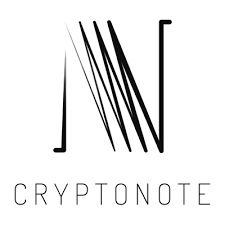
\includegraphics[width=0.20\textwidth]{Images/CryptoNote/cryptonote.png}
\end{wrapfigure}
The \emph{CryptoNote Technology} is designed to provide some of the most innovative privacy features predicated on advanced cryptography, an egalitarian approach towards decentralization and censorship-resistance. CryptoNote, as described in the Bitcoin forum~\cite{btcforum}, is the technology that allows creation of privacy-centric cryptocurrencies. The level of anonymity provided by CryptoNote isn't possible with Bitcoin code base by design. \emph{Bytecoin (BCN)} was the CryptoNote reference implementation, and \emph{Monero (XMR)} is based on BCN's code.

The CryptoNote protocol possesses significant algorithmic differences relating to blockchain obfuscation. One of the main features of CryptoNote, are \emph{ring signatures}~\cite{citeulike:14139412} that mask sender identities by mixing them and one-time keys that make transactions unlinkable. Their combined effect gives a high degree of anonymity without any extra effort on the part of the user.

Unlike Bitcoin, a user's funds are not held in the address he/she gives out to others. Instead, every time he/she receives a payment it goes to an unlinkable address generated with random numbers. When he/she decides to spend the funds in that one-time address, the amount will be broken down and the components will be indistinguishable from identical outputs in the blockchain.

For example if 556.44 XMR are sent, the protocol will break it down into 500 + 50 + 6 + 0.4 + 0.04 and a ring signature will be performed with other 500's, 50's, 6's, 0.4's, and 0.04's in the blockchain. Unlike the \emph{CoinJoin} mixing method~\cite{btcforum}, CryptoNote mixes outputs not transactions. This means no other senders need to be participating with some user at the same time or with the same amounts. Any arbitrary amount sent at any time can always be rendered fundamentally indistinguishable (a mathematical proof is given in the white paper~\cite{citeulike:14139412}).

The degree of anonymity is also a choice rather than decided by the protocol: do you want to be hidden as one among five or one among fifty? The size of the signature grows linearly as $\mathcal{O}(n+1)$ with the ambiguity, so greater anonymity is paid for, with higher fees to miners.

\subsection{Untraceable transactions} \label{sec:untraceable}
%\setlength{\intextsep}{0pt}
\begin{wrapfigure}[7]{L}{0.22\textwidth}
\centering

\includegraphics[width=0.22\textwidth]{Images/CryptoNote/untraceable.jpg}
\end{wrapfigure}
CryptoNote cryptographic scheme relies on the cryptographic primitive called a \emph{group signature}. First presented by D. Chaum and E. van Heyst~\cite{group}, it allows a user to sign his message on behalf of the group. The idea is actually simple. After signing the message the sender provides the keys of all the users of his group. A verifier is convinced that the real signer is a member of the group but cannot be exclusively identified.

However, this primitive required a trusted third party (Group Manager) who could trace the signer. The \emph{ring signature} was introduced by Rivest et al.~\cite{ring} and it was an autonomous scheme without anonymity revocation. Based on this work various modifications arose like \emph{linkable ring signature}~\cite{link1,link2,short}, a scheme that allowed to determine if two signatures were produced by the same group member, \emph{traceable ring signature}~\cite{traceable1,traceable2}, a scheme that limited anonymity (it is possible to trace the signer of two messages) and \emph{ad-hoc group signature}~\cite{ad-hoc1,ad-hoc2}. The last scheme focuses on the arbitrary group formation. The other schemes rather imply a fixed set of members.

Based on~\cite{traceable2} with a few modifications, in CryptoNote white paper~\cite{citeulike:14139412} is presented the \emph{one-time ring signature}. They weakened the traceability property and kept the linkability. That is needed because they wanted some user's public key to appear in many foreign verifying sets and from the private key to generate a unique anonymous signature. In case of a double spend attempt, these two signatures will be linked together. However, revealing the signer is not necessary.

Ring signatures are explained below. We will start with a normal signature scheme shown in \hyperref[fig:normal_sig]{figure}~\ref{fig:normal_sig}. Reproduced from CryptoNote~\cite{cryptonote}:
\vspace{0.5cm}
\begin{figure}[H]
  \centering
  \includegraphics[width=1 \columnwidth,keepaspectratio]{Images/CryptoNote/normal_sig.png}
  \caption{Normal signature: One participant, which allows one-to-one mapping.~\cite{cryptonote}}
  \label{fig:normal_sig}
\end{figure}

In \hyperref[fig:ring_sig]{figure}~\ref{fig:ring_sig} we show the ring signature concept.
\vspace{0.5cm}
\begin{figure}[H]
  \centering
  \includegraphics[width=1 \columnwidth,keepaspectratio]{Images/CryptoNote/ring_sig.png}
  \caption{Ring signature: Only proves that a signer belongs to a group.~\cite{cryptonote}}
  \label{fig:ring_sig}
\end{figure}

The result is shown in \hyperref[fig:result]{figure}~\ref{fig:result}. The reader can think of it as decentralized and trustless mixing.
\vspace{0.5cm}
\begin{figure}[H]
  \centering
  \includegraphics[width=1 \columnwidth,keepaspectratio]{Images/CryptoNote/result.png}
  \caption{High level of anonymity in cryptocurrency transactions.~\cite{cryptonote}}
  \label{fig:result}
\end{figure}

For an example of a complete CryptoNote transaction the reader is refered to  \hyperref[sec:cryptonote_transaction]{section}~\ref{sec:cryptonote_transaction}. Due to figure's size and complexity, it was improbable for us to manage to describe this example here, without compromising readability.

\subsection{Unlinkable transactions}
First, we should clarify the problem which is solved with unlinkability. Even if a transaction is untraceable, when the receiver posts his/her public address anyone can check all his/her incoming transactions (see \hyperref[fig:linkable]{figure}~\ref{fig:linkable}). A naive solution is to create a bunch of keys and addresses that can be sent privately to the payers (one distinct key per payer). This approach is highly problematical since it:
\begin{enumerate}[label=\alph*)]
  \item Deprives the receiver of the convenience of having a single public address
  \item Implies that the default use of the structure \textbf{DOES NOT} create unlinkable transactions
\end{enumerate}
\begin{figure}[H]
  \centering
  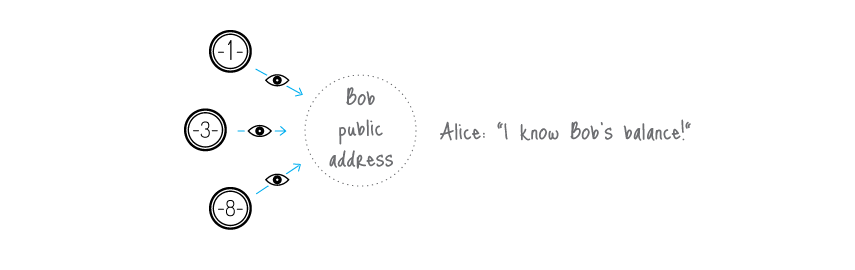
\includegraphics[width=0.9 \columnwidth,keepaspectratio]{Images/CryptoNote/linkable.png}
  \caption{Linkable transactions.~\cite{cryptonote}}
  \label{fig:linkable}
\end{figure}
\vspace{0.15cm}

CryptoNote solves this problem. It creates automatically and by default multiple unique one-time keys, derived from the single public key, for each peer-to-peer payment. The solution lies in a clever modification of the Diffie-Hellman exchange protocol~\cite{Diffie:2006:NDC:2263321.2269104}. Originally, it allows two parties to produce a common secret key derived from their public keys. In CryptoNote protocol the sender uses the receiver's public address and his own random data to compute a one-time key for the payment.

The sender can produce only the public part of the key, whereas only the receiver can compute the private part; hence the receiver is the only one who can release the funds after the transaction is committed. He/she only needs to perform a single-formula check on each transaction to establish if it belongs to him/her. This process involves his/her private key, therefore no third party can perform this check and discover the link between the one-time key generated by the sender and the receiver's unique public address.
\begin{figure}[ht]
  \centering
  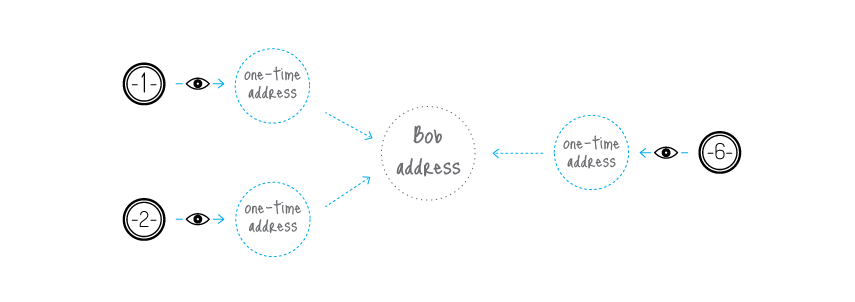
\includegraphics[width=0.9 \columnwidth,keepaspectratio]{Images/CryptoNote/unlinkable.png}
  \caption{Unlinkable transactions.~\cite{cryptonote}}
  \label{fig:unlinkable}
\end{figure}
\vspace{0.15cm}

An important part of CryptoNote is the use of random data by the sender. It always results in a different one-time key, even if the sender and the receiver both remain the same for all transactions (that is why the key is called "one-time"). Moreover, even if they are both the same person, all the one-time keys will also be absolutely unique.

\subsubsection{Stealth addresses} \label{sec:stealth}
%\setlength{\intextsep}{0pt}
\begin{wrapfigure}[6]{L}{0.3\textwidth}
\centering
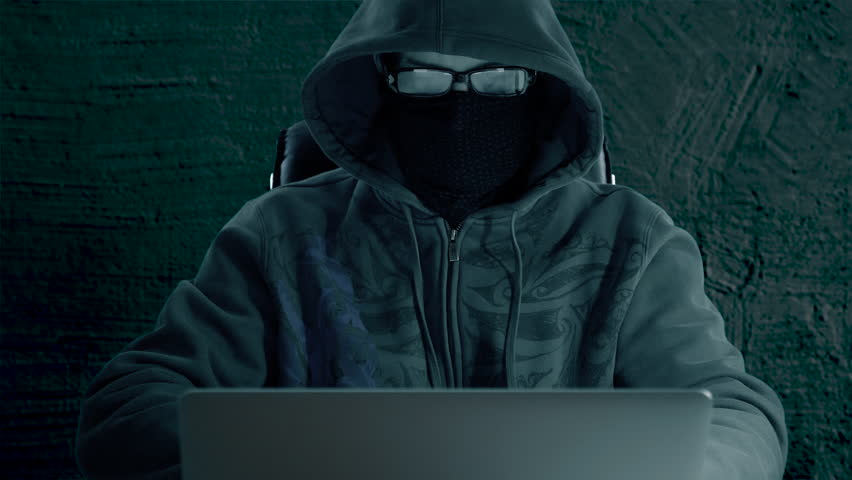
\includegraphics[width=0.30\textwidth]{Images/CryptoNote/stealth.jpg}
\end{wrapfigure}
The structure of the above concept is inherited in all CryptoNote projects. But the details of each implementation may differ. What we will present here is the implementation details of unlinkability, as found in the Monero project. The reader can find all the information of this section and more in CryptoNote paper~\cite{citeulike:14139412} and Monero project's code~\cite{monerocode}. An additional valuable source of information and interactive conversation venue that the reader is refered to is Monero stack exchange forum~\cite{stackexchange}. The implementation of CryptoNote's unlinkable transactions in Monero project is mentioned as \emph{stealth addresses} or \emph{subaddresses}.

Stealth address technology originated from CryptoNote technology, but Bitcoin (e.g. \emph{libbitcoin}) and its altcoins can also implement stealth addresses. For Bitcoin and its altcoins, stealth addresses must be explicitly supported by the sender's and recipient's wallets, but such support is implicit to CryptoNote wallets.
\begin{figure}
  \begin{verbatim}
 vJmsp9MxWMj6jiUg8Rejh23pqRCthWQhwtUKvmLw2kcE83AHer1MchTN4DVacHt
 43r8hSKBQpjPuqYDKuKgyVBkGkUdcsNAdnk2aZW
  \end{verbatim}
  \caption{Bitcoin stealth address.}
  \label{fig:btcstealth}
\end{figure}

For Bitcoin, stealth addresses are a bit longer than normal Bitcoin addresses (see \hyperref[fig:btcstealth]{figure}~\ref{fig:btcstealth}). However, the transactions associated with a stealth address looks no different than normal transactions on the Bitcoin blockchain. Stealth addresses contain one public \emph{view} (in CryptoNote vernacular) or \emph{scan} (in Bitcoin vernacular) key, and one or more \emph{spend} public keys. These keys are always encoded in a stealth address to support the first portion of Diffie-Hellman key exchange~\cite{Diffie:2006:NDC:2263321.2269104}. Bitcoin's public/private key pairs are derived from the \emph{secp256k1} elliptic curve~\cite{secg}, while CryptoNote uses \hyperref[sec:ed25519]{\emph{Ed25519}}~\cite{curve25519} (see \hyperref[sec:ed25519]{section}~\ref{sec:ed25519}) derived public/private key pairs.

One can publish their stealth address on a business card, and sustain their privacy when funds are sent to a dynamically computed destination address by the sender of funds. Stealth addresses essentially put the onus of dynamic address calculation, typically associated with a recipient's hierarchical deterministic (HD) wallet, on the sender's wallet. One stealth address is functionally akin to an HD wallet account, and can thus be used over and over for many fund transfers. Stealth addresses provide confidentiality for the recipient of transaction pairs that utilize information from a stealth address.

So, simplifying a bit, in Bitcoin if there is one Bitcoin associated to the public key $P$ and if Bob knows the corresponding private key $x$ such that $P = xG$\footnote{$G$ is the generator for the algebraic ring that is the base of the key construction. For our purpose, it suffices to think $G$ as a parameter of the user's existence in the Monero network, which is public and thus available to anyone.}, then he can spend the Bitcoin by submitting a message (transaction) to the network signed with $x$.

There is one privacy issue, though: if Bob keeps using the same $P$ to receive Bitcoins, then any observer will be able to see all payments were made to the same entity that controls $P$ (Bob). This is the problem that stealth addresses solve.
\pagebreak

Stealth addresses innately perform the first half of a Diffie-Hellman key exchange~\cite{Diffie:2006:NDC:2263321.2269104} when a sender of funds receives a stealth address. In Bitcoin, two blockchain transactions are required to complete the sending of funds to a stealth address that belongs to the recipient of funds.

Since it is operationally improbable for two users' wallets to communicate directly to each other, the first transaction is a persistent \verb|OP_RETURN| transaction that is used to complete the second half of a Diffie-Hellman key exchange. The second transaction is the actual sending of funds to a dynamically calculated destination address that is strongly based upon an ephemeral random number generator in the sender's wallet.

The second half of the Diffie-Hellman key exchange, the \verb|OP_RETURN|, allows the recipient's wallet of a stealth transaction to dynamically calculate the private redemption key associated with a particular transaction to redeem the funds at a later date.

Stealth addresses can be extended to support multisig. This is a multisig capability that is more inherent to Bitcoin than CryptoNote.

In the context of stealth addresses, addresses are now composed of two public keys, and the coins sent to Bob will not be sent to his stealth address on the blockchain, rather the stealth address will be used by the sender to produce fresh new Bitcoin addresses for every new transaction. These new addresses, even though generated by the sender (Alice) and unknown to Bob until the transaction is made, will nonetheless be controlled by Bob! Here is how it works:

Bob creates two pairs of private and public keys. Let's denote them by $(a,A)$ and $(b,B)$, where by definition
\begin{equation}
  A = aG \quad \mbox{ and } \quad B = bG
\end{equation}
Bob makes the pair of public keys $(A,B)$ available to the network; this will be his stealth address.

Alice wishes to send one Bitcoin to Bob. She wants to assign one Bitcoin to a public key $P$ such that Bob knows $x$ and $P = xG$. She will construct such $P$ using Bob's stealth address by using a hashing function $\mathcal{H}$, choosing a random big number $r$, and setting
\begin{equation}
  P = \mathcal{H}(rA)G + B
\end{equation}
Then, Alice sends the Bitcoin to $P$ and the transaction is broadcast along with $R = rG$ (but not $r$, which can't be recovered from $R$).

In order to get the money, Bob has to keep listening to the network for all new transactions and check whether one or more of these transactions are money that he should receive. When he sees Alice's transaction, he checks if $x := \mathcal{H}(aR)+b$ and realizes that:
\begin{align*} \label{eq:checkstealth}
  xG &= (\mathcal{H}(aR)+b)G \\
     &= \mathcal{H}(aR)G+bG \\
     &= \mathcal{H}(arG)G+B \\
     &= \mathcal{H}(raG)G+B \\
     &= \mathcal{H}(rA)G+B \\
     &= P
\end{align*}
\pagebreak

Bob can reconstruct $x$ such that $P = xG$ and is therefore the owner of the Bitcoin! Notice that neither Alice nor any observer has the ability to derive $x$ (because they don't know $a$ and $b$), and that besides Alice and Bob no one knows that $(x,P)$ was generated from Bob's stealth address (because they don't know $r$).

Ignoring middleman snooping on IP addresses associated with stealth address transaction pairs, only the two core parties involved in a transaction pair will know any identity details associated with sending funds to a stealth address. Hence, the need for \hyperref[sec:Kovri]{Kovri I2P technology} (see \hyperref[sec:Kovri]{section}~\ref{sec:Kovri}). So, stealth transactions by themselves don't provide 100\% anonymity protection. Also Confidential Transactions (CT) technology is needed by Bitcoin to mask details about the amount transferred by a transaction.

Note that, as mentioned, this protects Bob's privacy, but it is still visible to the network that Alice, the entity that used to control that Bitcoin, made a transaction. In order to obfuscate that action, Monero implements the use of Ring Signatures~\cite{ringCT}, which will allow Alice to, instead of directly signing the transaction, produce a proof that her or several other people, did send a coin to Bob.

To sum up, in Monero, coins are received to a unique one-time stealth address. The formula for stealth addresses, is as follows:
\begin{equation}
  P = \mathcal{H}(rA)G + B
\end{equation}
%
Where:
\begin{description}
  \item [G] The standard \emph{Ed25519} base point
  \item [A] Bob's public view key
  \item [B] Bob's public spend key
  \item [r] The new random scalar Alice chose for this transaction
  \item [$\mathcal{H}$] A hashing algorithm that returns a scalar (i.e., the hash output is interpreted as an integer and reduced modulo $l$)
  \item [P] The final stealth address (one-time output key, the destination where funds will actually be sent)
\end{description}
So, in a nutshell:
\begin{itemize}
  \item \emph{Stealth addresses} take care of \textbf{recipient's} privacy.
  \item \emph{Ring Signatures} take care of \textbf{sender's} privacy.
\end{itemize}

An \hyperref[sec:construction]{example} is presented in the \hyperref[sec:construction]{Appendix}~\ref{sec:construction} of this thesis. There, the reader can find a real world construction of a Monero stealth address.
\clearpage
\pagebreak

\subsection{Stealth address construction} \label{sec:construction}
Here is a functional example for deriving a Monero stealth address. Here we will examine the developer mechanics not cryptographic theory. Results below duplicate functionality that is part of \emph{Crypto Note Test Address}~\cite{teststealth}.

It is worth noting custom \verb|bytes_to_words|, \verb|sc_reduce32|, and \verb|secret_key_to_| \verb|public_key| executables (coded in C or C++) below were named after Monero's functions that yielded output results. C++ coding insights came from \verb|main.cpp|. The \verb|bx| command line is bitcoin-explorer, see~\cite{bx}.

Monero's \verb|secret_key_to_public_key()| functionality is using \hyperref[sec:ed25519]{\emph{Ed25519}} (see \hyperref[sec:ed25519]{section}~\ref{sec:ed25519}) technology but not in an inclusive way. Only the necessary computations for the production of stealth addresses are implemented. Results are different from \emph{Tor}~\cite{tor} test vectors results that custom executables utilizing \emph{libsodium} and \emph{ed25519-donna} yield, but Monero C/C++ code results match that from \emph{Crypto Note Test Address}. Let us see the components and the calculations that take place in order to construct a stealth address.

The example that is presented here was posted by user \verb|skaht| on Monero stack exchange forum~\cite{stackexchange}. The calculations were checked and confirmed.
\begin{itemize}
  \item 256-bit hexadecimal-encoded seed is assumed to be:
  \begin{verbatim}
  198584347013dd91832be3d82529437db7cc8e1850e559cdd3872b29
  ca819601
  \end{verbatim}
  \item Electrum mnemonic words\footnote{These are the words that a wallet owner should remember in order to restore his wallet, if he forgets his password.} corresponding to seed\\
  (\verb|./bytes_to_words <above seed>|)
  \begin{verbatim}
  $ ./bytes_to_words 198584347013dd91832be3d82529437db7cc8
  e1850e559cdd3872b29ca819601
  \end{verbatim}
  \begin{tcolorbox}[colback=blue!5!white,colframe=blue!65!black,title=Output:]
    wallets drinks insult popular fall textbook scoop apology unsafe fifteen cuffs pimple roster nerves pixels upstairs academy sprig eclipse leopard peeled faxed gutter happens roster
  \end{tcolorbox}
  \item Private spend key calculation\\
  (\verb|./sc_reduce32 <private spend key>|)
  \begin{verbatim}
  $ ./sc_reduce32 198584347013dd91832be3d82529437db7cc8e185
  0e559cdd3872b29ca819601
  \end{verbatim}
  \begin{tcolorbox}[colback=blue!5!white,colframe=blue!65!black,title=Output:]
    \small{198584347013dd91832be3d82529437db7cc8e1850e559cdd3872b29ca819601}
  \end{tcolorbox}
  \item Private view key calculation\\
  (\verb|./keccak|\footnote{Hash function.}\verb=<private spend key> | ./sc_reduce=)
  \begin{verbatim}
  $ ./keccak 198584347013dd91832be3d82529437db7cc8e1850e559c
  dd3872b29ca819601
  $ ./sc_reduce32 <the keccak output>
  \end{verbatim}
  \begin{tcolorbox}[colback=blue!5!white,colframe=blue!65!black,title=Output:]
    \footnotesize{889DA12A88D36BCE0966AB1A79125779DD1F2FC6F1145DE131FD52A5B468796D}
    \tcblower
    \small{faa5defce980fdbd03b9dd4841371dfcdc1f2fc6f1145de131fd52a5b468790d}
  \end{tcolorbox}
  \item Public spend key calculation\\
  (\verb|./secret_key_to_public_key <private spend key>|)
  \begin{verbatim}
  $ ./secret_key_to_public_key 198584347013dd91832be3d82529437
  db7cc8e1850e559cdd3872b29ca819601
  \end{verbatim}
  \begin{tcolorbox}[colback=blue!5!white,colframe=blue!65!black,title=Output:]
    \small{b66991d7d7c68513533d0560f820d75adfb0911487ba62274b759f7b3ccd4a90}
  \end{tcolorbox}
  \item Public view key calculation\\
  (\verb|./secret_key_to_public_key <private view key>|):
  \begin{verbatim}
  $ ./secret_key_to_public_key faa5defce980fdbd03b9dd4841371
  dfcdc1f2fc6f1145de131fd52a5b468790d
  \end{verbatim}
  \begin{tcolorbox}[colback=blue!5!white,colframe=blue!65!black,title=Output:]
    \small{3c450f27cd6849d9130addb2c566d910c5ef9bf4cecaed547004496fda52a4ff}
  \end{tcolorbox}
\end{itemize}

Note that the calculation of the stealth address (hexadecimal format) is:
\begin{verbatim}
    prefix + public_spend_key + view_public_key +
                                      keccak_checksum_postfix
\end{verbatim}
\clearpage
\pagebreak

The \verb|prefix| in Monero addresses is always $12$ and is a marking of a Monero address. In this context the character \verb|+| is used to mark concatenation of strings. The \verb|keccak_checksum_postfix| computation is:
\begin{itemize}
  \item Stealth address checksum calculation (\verb|./keccak <almost an address>|):
  \begin{verbatim}
$ ./keccak 12 +
b66991d7d7c68513533d0560f820d75adfb0911487ba62274b759f7b3
ccd4a90 +
3c450f27cd6849d9130addb2c566d910c5ef9bf4cecaed547004496fd
a52a4ff
  \end{verbatim}
  \begin{tcolorbox}[colback=blue!5!white,colframe=blue!65!black,title=Output:]
    \footnotesize{ADD568169DBF2C6D3F595EE8610A189955BECD1EDF150627CBF2F2C49B0AEA71}
  \end{tcolorbox}
  \item So, the hexadecimal format of a Monero stealth address is:
  \begin{verbatim}
12b66991d7d7c68513533d0560f820d75adfb0911487ba62274b759f7
b3ccd4a903c450f27cd6849d9130addb2c566d910c5ef9bf4cecaed54
7004496fda52a4ffADD56816
  \end{verbatim}
\end{itemize}

In order to convert a hexadecimal representation of a stealth address in base58 format we calculate the base58 format of each 8 bytes and concatenate the results (presented between brackets). For the conversion, we used \verb|bx| (bitcoin explorer~\cite{bx}):

\begin{enumerate}
  \item \verb|$ bx base58-encode 12b66991d7d7c685| ($\rightarrow$ \verb|48Y3H2eSZ6C|)
  \item \verb|$ bx base58-encode 13533d0560f820d7| ($\rightarrow$ \verb|4EUjY1B5viS|)
  \item \verb|$ bx base58-encode 5adfb0911487ba62| ($\rightarrow$ \verb|GCbCLPcmMiy|)
  \item \verb|$ bx base58-encode 274b759f7b3ccd4a| ($\rightarrow$ \verb|7aD69yqUsaH|)
  \item \verb|$ bx base58-encode 903c450f27cd6849| ($\rightarrow$ \verb|R8GLE3rvSwr|)
  \item \verb|$ bx base58-encode d9130addb2c566d9| ($\rightarrow$ \verb|dJtpZYG1peC|)
  \item \verb|$ bx base58-encode 10c5ef9bf4cecaed| ($\rightarrow$ \verb|3oipCqfUvCc|)
  \item \verb|$ bx base58-encode 547004496fda52a4| ($\rightarrow$ \verb|F89i86kuEjV|)
  \item \verb|$ bx base58-encode ffADD56816| ($\rightarrow$ \verb|Vr5GCdj|)
\end{enumerate}

Finally, we get the Monero stealth address:
\vspace{0.3cm}
\begin{tcolorbox}[colback=green!5!white,colframe=green!65!black]
  \small{48Y3H2eSZ6C4EUjY1B5viSGCbCLPcmMiy7aD69yqUsaHR8GLE3rvSwrdJtpZYG\\
  1peC3oipCqfUvCcF89i86kuEjVVr5GCdj}
\end{tcolorbox}
\clearpage
\pagebreak

\subsection{Double-spending proof}
Fully anonymous signatures would allow spending the same funds many times which, of course, is incompatible with any payment system's principles. The problem can be fixed and here we reproduce the description of this solution, as presented in~\cite{cryptonote}.

A ring signature is actually a class of crypto-algorithms with different features. The one CryptoNote uses is the modified version of the \emph{traceable ring signature}~\cite{traceable2}. In fact, they transformed traceability into linkability. This property restricts a signer's anonymity as follows: if he/she creates more than one ring signature using the same private key (the set of foreign public keys is irrelevant), these signatures will be linked together which indicates a double-spending attempt.

To support linkability CryptoNote introduced a special marker being created by a user while signing, which they called a \emph{key image}. It is the value of a cryptographic one-way function of the secret key, so in mathematical terms it is actually an image of this key. One-wayness means that, given only the key image, it is impossible to recover the private key.

On the other hand, it is computationally impropable to find a collision (two different private keys, which have the same image). Using any formula, except for the specified one, will result in an unverifiable signature. All things considered, the key image is unavoidable, unambiguous and yet an anonymous marker of the private key.
\vspace{0.3cm}
\begin{figure}[H]
  \centering
  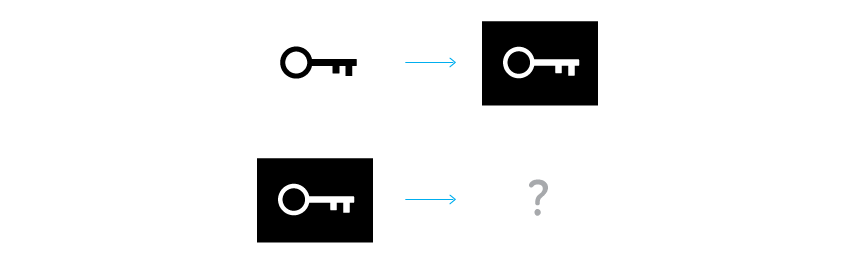
\includegraphics[width=1 \columnwidth,keepaspectratio]{Images/CryptoNote/key_image.png}
  \caption{Key image via one-way function.~\cite{cryptonote}}
  \label{fig:key_image}
\end{figure}
\vspace{0.2cm}

All users keep the list of the used key images (compared to the history of all valid transactions, it requires an insignificant amount of storage) and immediately reject any new ring signature with a duplicate key image. It will not identify the misbehaving user, but it does prevent any double-spending attempts, caused by malicious intentions or software errors.
\begin{figure}[H]
  \centering
  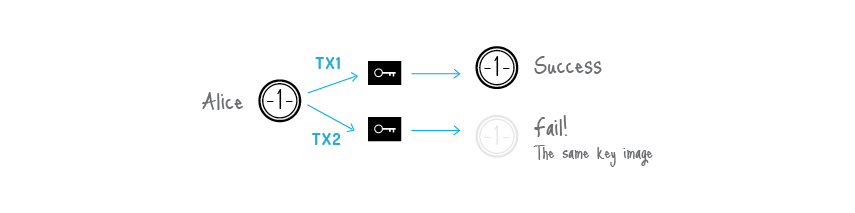
\includegraphics[width=1.2 \columnwidth,keepaspectratio]{Images/CryptoNote/double_spending.png}
  \caption{Double-spending check.~\cite{cryptonote}}
  \label{fig:double_spending}
\end{figure}
\vspace{0.2cm}

\subsection{Blockchain analysis resistance}
We reproduce from~\cite{cryptonote} the reasons, why blockchain analysis in Monero project is not something that can be achieved.

There are many academic papers dedicated to the analysis of the Bitcoin's blockchain. Their authors trace the money flow, identify the owners of coins, determine wallet balances and so on. The ability to make such analysis is due to the fact that all the transfers between addresses are transparent: every input in a transaction refers to a unique output. Moreover, users often re-use their old addresses, receiving and sending coins from them many times, which simplifies the analyst's work. It happens unintentionally: if one has a public address (for example, for donations), one is sure to use this address in many inputs and transactions.

CryptoNote is designed to mitigate the risks associated with key re-use and one-input-to-one-output tracing. Every address for a payment is a unique one-time key, derived from both the sender's and the recipient's data. It can appear twice with a probability of a 256-bit hash collision. As soon as you use a ring signature in your input, it entails the uncertainty: which output has just been spent?

Trying to draw a graph with addresses in the vertices and transactions on the edges, one will get a tree: a graph without any cycles (because no key/address was used twice). Moreover, there are billions of possible graphs, since every ring signature produces ambiguity. Thus, you can't be certain from which possible sender the transaction-edge comes to the address-vertice. Depending on the size of the ring you will guess from "one out of two" to "one out of a thousand". Every next transaction increases the entropy and creates additional obstacles for an analyst.

\subsection{More about CryptoNote}
There are several noteworthy details about CryptoNote and several implementation details of this protocol in the Monero project. However, it would be unproductive and it would harm the readability of this thesis to describe every aspect of this protocol. We believe that the reader has now a good understanding of the backbone of Monero's privacy and anonymity features. Nevertheless, before we start the \hyperref[ch:cryptonight]{CryptoNight} description (see \hyperref[ch:cryptonight]{section}~\ref{ch:cryptonight}) we will elaborate on some additional details about CryptoNote. Reproduced from~\cite{cryptonote}:

\subsubsection{Adaptive limits}
A decentralized payment system must not depend on a single person's decisions, even if this person is a core developer. Hard constants and magic numbers in the code deter the system's evolution and therefore should be eliminated (or at least be cut down to the minimum).

Every crucial limit (like max block size or min fee amount) should be re-calculated based on the system's previous state. Therefore, it always changes adaptively and independently, allowing the network to develop on it's own. CryptoNote has the following parameters which adjust automatically for each new block:
\clearpage
\pagebreak

\begin{description}
  \item [Difficulty] The general idea of our algorithm is to sum all the work that nodes have performed during the last 720 blocks and divide it by the time they have spent to accomplish it. The measure of the work is the corresponding difficulty value for each of the blocks. The time is calculated as follows: sort all the 720 timestamps and cut-off 20\% of the outliers. The range of the rest 600 values is the time which was spent for 80\% of the corresponding blocks.
  \item [Maximum block size] Let $MN$ be the median value of the last $N$ blocks sizes. Then the \emph{hard-limit} for the size of accepting blocks is $2 \cdot MN$. It averts blockchain bloating but still allows the limit to slowly grow with the time, if necessary. Transaction size does not need to be limited explicitly. It is bounded by the size of the block.
\end{description}

\subsubsection{Smooth emission}
In the CryptoNote description~\cite{cryptonote} one can find the following; the upper bound for the overall amount of all digital coins is also digital:
\begin{equation}
  \mbox{MSupply } = 264 − 1 \mbox{ atomic units}
\end{equation}

This is a natural restriction based only on implementation limits, not on intuition like "$N$ coins ought to be enough for everybody". To make the emission process smoother, CryptoNote uses the following formula for block rewards:
\begin{equation}
  \mbox{BaseReward } = (\mbox{MSupply } - A) >> 18
\end{equation}
where $A$ is the amount of previously generated coins. It gives a predictable growth of the money supply without any breakpoints.

During our research, we found the above description peculiar and confusing. After a while and some forum conversations, we understood that the actual implementation restriction is that a single output cannot have an amount greater than $2^{64} − 1$ atomic units (which is $1.84 \cdot 10^{31}$ XMR).

Therefore the restriction that the above feature is referring to, is about individual outputs and not the total sum of all outputs that can exist on the blockchain.
\vspace{0.2cm}

This is currently an implementation limitation related to Monero's \hyperref[sec:bulletproofs]{\emph{bulletproofs}}~\cite{getmonero} (see \hyperref[sec:bulletproofs]{section}~\ref{sec:bulletproofs}) which proves that amounts are not negative, by proving they are less than $2^{64}$. Because Monero units are expressed as positive integers which are subject to modular arithmetic, a very high number can be equivalent to a negative number when added to another Monero amount, which is why this "less than" check proves the number is not effectively negative.

It's easy for this limit to be increased, if necessary, in the future (it's extremely unlikely to be necessary). Note that this observation is specifically related to theoretical limitations. It may be possible that certain Monero wallet implementations also store amounts using a data storage technique that would prevent numbers larger than $2^{64}$ from being stored.
\clearpage
\pagebreak

\subsubsection{CryptoNote Transaction} \label{sec:cryptonote_transaction}
%
Here we will present a complete CryptoNote transaction from Bob to Carol. Again reproduced from CryptoNote~\cite{cryptonote}, we will subjoin an example and a figure showing the details. The example below is illustrated in \hyperref[fig:transaction]{figure}~\ref{fig:transaction}, in the next page.

Bob decides to spend an output, which was sent to the one-time public key. He needs Extra \textbf{(1)}, TxOutNumber \textbf{(2)}, and his Account private key \textbf{(3)} to recover his one-time private key \textbf{(4)}.

When sending a transaction to Carol, Bob generates its Extra value by random \textbf{(5)}. He uses Extra \textbf{(6)}, TxOutNumber \textbf{(7)} and Carol's Account public key \textbf{(8)} to get her Output public key \textbf{(9)}.

In the input Bob hides the link to his output among the foreign keys \textbf{(10)}. To prevent double-spending he also packs the Key image, derived from his One-time private key \textbf{(11)}.

Finally, Bob signs the transaction, using his One-time private key \textbf{(12)}, all the public keys \textbf{(13)} and Key Image \textbf{(14)}. He appends the resulting Ring Signature to the end of the transaction \textbf{(15)}.
\clearpage
\pagebreak

\begin{figure}[ht]
  \centering
  \includegraphics[scale=0.31, angle=90, keepaspectratio]{Images/CryptoNote/transaction.png}
  \caption{A sample transaction from Bob to Carol.~\cite{cryptonote}}
  \label{fig:transaction}
\end{figure}
\clearpage
\pagebreak

\subsubsection{CryptoNote elliptic curve} \label{sec:ed25519}
The elliptic curve \emph{ed25519} is both a signature scheme and a use case for Edwards form Curve25519~\cite{eddsa}. EdDSA (\emph{Edwards-curve Digital Signature Algorithm}) generalises this signature scheme to any curve in Edwards form.

\emph{Curve25519} first arrived in 2006~\cite{curve25519}, a few years before the Edwards normal form papers on elliptic curves. Montgomery curves, the form of curve used for Curve25519, was originally used to speed up elliptic curve factorisation~\cite{montgomery}. The original proposal for Curve25519 was for use as a Diffie-Hellman (key exchange) protocol~\cite{Diffie:2006:NDC:2263321.2269104}. This is still its use and is now often called \emph{X25519}.

Later, Edwards came up with his own form of elliptic curve~\cite{edward}. Daniel J. Bernstein, Tanja Lange et al. researched these forms and realised they too were fast, especially for signatures and we got Ed25519~\cite{eddsa} using the Edwards form of Curve25519. So far, we have the following nomenclature:
\begin{description}
  \item [Curve25519, Curve41417, Ed448-Goldilocks] generally the name of the curve itself.
  \item [X25519, X448, X41417] Diffie-Hellman key exchange schemes using the above curve.
  \item [EdDSA, Ed25519, Ed448] The first being the generic Edwards variant of DSA, plus other fixes, the others being specific instances matched to their curve names.
\end{description}
Confusingly, Open Whisper Systems came up with \emph{XEdDSA}~\cite{signal}. To quote them:
\begin{verbatim}
  XEdDSA enables use of a single key pair format for both elliptic
  curve Diffie-Hellman and signatures.
\end{verbatim}

Hence, \emph{X EdDSA} is taken to mean "exchange and EdDSA" of the given curve. In this instance, the key exchange part still happens using the montgomery form of the curve, but the signature part (EdDSA) uses the same curve in Edwards form.
\pagebreak

\section{Monero vs CryptoNote}
The reader understands now that the backbone for Monero's anonymity and privacy features is CryptoNote protocol. However, there are some differences. One that was already pointed out is the \hyperref[sec:stealth]{\emph{stealth address}} feature. We have noted in \hyperref[sec:stealth]{section}~\ref{sec:stealth} that the Monero stealth address implementation is unique. Other CryptoNote projects do not share exactly the same calculations.

Moreover, Monero is actively developed as it is one of the most successful cryptocoin projects and several additions have been made since its first introduction to the world. Its backbone is still the CryptoNote protocol but in this section we will mention additional features that strengthen the anonymity and privacy goals of the project.

\subsection{RingCT}
In the \hyperref[sec:untraceable]{Section}~\ref{sec:untraceable} we mentioned \emph{one-time ring signatures} that were presented in CryptoNote white paper.

In 2015, Shen Noether wrote a paper using a technique, introduced by Bitcoin Core developer Gregory Maxwell in~\cite{elements}, of using a commitment scheme to hide the amount of a transaction. The paper introduced \emph{RingCT (Ring Confidential Transactions)}~\cite{ringCT}. This signature scheme is called \emph{A Multi-layered Linkable Spontaneous Anonymous Group signature} and that is how transaction amounts are hidden in Monero. Reproducing from~\cite{getmonero}:

\begin{verbatim}
  RingCT was implemented in block #1220516 in January 2017.
  After September 2017, this feature became mandatory for all
  transactions on the network.
\end{verbatim}
For further information the reader is refered to Shen Noether's paper~\cite{ringCT}.

The transaction structure remains similar to the structure in \hyperref[sec:Bitcoin]{Bitcoin}: every user can choose several independent incoming payments (transactions outputs), sign them with the corresponding private keys and send them to different destinations. Contrary to Bitcoin’s model, where a user possesses unique private and public keys, in the proposed model a sender generates a one-time public key based on the recipient’s address and some random data.

In this sense, an incoming transaction for the same recipient is sent to a one-time public key (not directly  to a unique  address) and only the recipient can recover the corresponding private part to redeem his funds (using his unique private key). The recipient can spend the funds using a ring signature, keeping his ownership and actual spending anonymous.
\clearpage
\pagebreak

\subsection{Bulletproofs} \label{sec:bulletproofs}
%\setlength{\intextsep}{0pt}
\begin{wrapfigure}[7]{L}{0.2\textwidth}
\centering
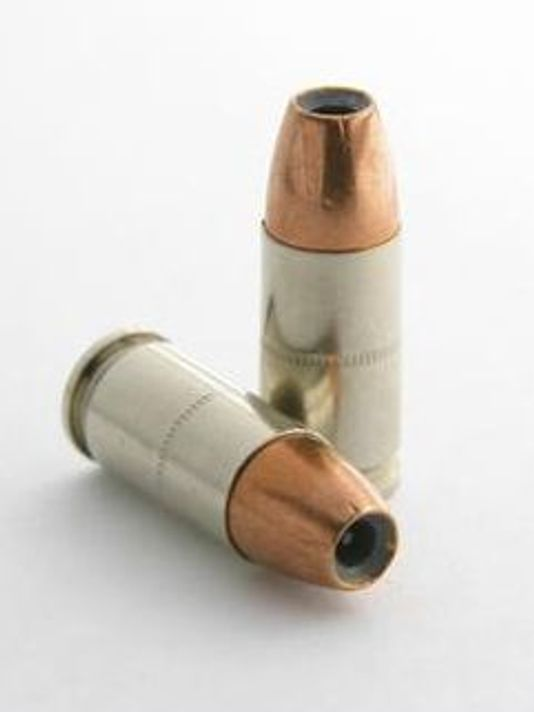
\includegraphics[height=0.23\textwidth]{Images/Monero/bullet.jpg}
\end{wrapfigure}
Starting in 2018, Monero began testing yet another highly sophisticated piece of cryptographic magic: \emph{bulletproofs}~\cite{bulletproofs}. This technology is intended to address one of the main drawbacks of \emph{RingCT}~\cite{ringCT}: the size of the \emph{zero-knowledge range proofs} this scheme produces. \emph{Bulletproofs} are a big deal, as they can increase the privacy of digital currency transactions and at the same time dramatically decrease their size. The scalability of confidential transactions have been a significant hurdle for the \$1 billion blockchain, with users long suffering high transaction fees as well as an ever-increasing cost of storage for running a full node.

\subsubsection{History}
After working on the \emph{Confidential Transactions} scheme~\cite{ringCT}, Greg Maxwell, Andrew Poelstra and Pieter Wuille teamed up with researchers from the Stanford Applied Cryptography Group to make it more efficient. Their research focused on applying a \emph{non-interactive zero knowledge proof (NIZKP)} system~\cite{0_knowledge} to aggregate all the range proofs of a Confidential Transaction and collectively prove their validity.

For context, the basic concept behind a zero-knowledge proof is to cryptographically prove that something exists, without knowing what that something is. This is achieved through a set of challenges that, if completed successfully, can statically prove that a party has a secret, without knowing what that secret is. This is the technology employed by Zcash~\cite{zcash} to entirely shield senders, receivers and the amount of ZEC (Zcash cryptocoin) sent in a transaction.

Zero-Knowledge proofs are an amazing and counter-intuitive cryptographic concept, first proposed by Goldwasser, Micali and Rackoff~\cite{0_knowledge} in a paper that introduced the idea of \emph{interactive proof} systems. The literature is extensive and if the reader wants to learn about the more modern and practical references and implementations, he/she can find the ZKP Science website~\cite{zkp_science} very useful.

The NIZKP system proposed by the bulletproof white paper~\cite{bulletproofs} has both benefits and drawbacks. On one hand, the use of \emph{NIZKP bulletproofs} does not require a trusted setup for parameter generation, like Zcash’s Powers of Tau ceremony~\cite{powers_of_tau}. On the other hand, the verification of a bulletproof is more time consuming.

\subsubsection{Details}
In order to understand bulletproofs, the reader needs to understand what a \emph{range proof} is. According to~\cite{getmonero}:
\begin{verbatim}
  A range proof allows anyone to verify that a commitment
  represents an amount within a specified range, without
  revealing anything else about its value.
\end{verbatim}

Monero uses a range proof in RingCT~\cite{ringCT} to secure the amount being sent in a transaction. Without range proofs, the amount sent could be hidden, but a sender could cheat by making coins out of thin air. Range proofs prevent this from happening. Bulletproofs achieve this goal more efficiently.
\pagebreak

\noindent From the whitepaper~\cite{bulletproofs}:
\begin{verbatim}
  [...] a new non-interactive zero-knowledge proof protocol
  with very short proofs and without a trusted setup; the
  proof size is only logarithmic in the witness size.
  Bulletproofs are especially well suited for efficient
  range proofs on committed values [...]
\end{verbatim}

Beyond improving the privacy assumptions within confidential transactions~\cite{ringCT}, bulletproofs have a much lower fingerprint (or size) relative to the proof systems used in blockchain networks today. In fact, much like \emph{SegWit}~\cite{segwit}, bulletproofs can be seen as an approach to vertical scalability as they can greatly decrease the size of a cryptographic proof from over 10kB to less than 1kB.

The bulletproof white paper~\cite{bulletproofs} focused on applying NIZKPs to the Bitcoin blockchain and stated that, if implemented, total size of Bitcoin’s UTXO\footnote{Unspent Transaction Output. UTXOs are processed continuously and are responsible for beginning and ending each transaction. Confirmation of transaction results lies in the removal of spent coins from the UTXO database. But a record of the spent coins still exists on the ledger.~\cite{investopedia}} set would be only 17 GB (compared to 160 GB) if confidential transactions were to be implemented.

It’s worth noting that bulletproofs don’t actually contribute to privacy itself. Rather, they simply ensure that the information stored within a confidential transaction doesn’t contain any false information. Pseudonymous Monero cryptographer Sarang Noether, who assisted with the bulletproofs' integration, told CoinDesk~\cite{coindesk}:
\begin{verbatim}
  They’re not about anonymity; they are about assuring that
  the other stuff we do for anonymity works correctly.
\end{verbatim}

Under the previous range proof format, the size of XMR transactions scale mostly linearly depending on the number of outputs (1 output = 7kB, 2 outputs = 13kB). Under bulletproofs, transaction sizes scale logarithmically instead (1 output = 2kB, 2 outputs = 2.5kB). The size of a bulletproof increases only logarithmically with both the size of the range and the number of outputs. Reproducing from~\cite{getmonero}:
\begin{verbatim}
  This gives us two related types of bulletproofs: single-output
  and multiple-output. A transaction with multiple outputs can
  either include several single-output proofs or one multiple-output
  proof (which is smaller than the separate proofs).
\end{verbatim}

Therefore, this technology has the potential to greatly contribute to Monero’s scalability. However, one problem arose. Again, reproduced from~\cite{getmonero}:
\begin{verbatim}
  [...] an attacker could pack a transaction with many outputs;
  this tiny transaction would require low fees but would be
  computationally expensive to verify, opening the door to
  denial-of-service attacks. Because of this, we will need to
  adjust the fee structure away from transaction size and take
  into account the verification scaling.
\end{verbatim}
They explain that this means that the fees will scale properly and in a safe way. It does not mean that fees go up.
\pagebreak

The space savings granted by bulletproofs may also enable the implementation of additional obfuscation mechanisms. It is noteworthy that increasing the mandatory number of outputs in a transaction can make it significantly harder to trace balances by analyzing the blockchain. Decoys are used in ring signature inputs, but not in a transaction’s outputs. Implementing a system of decoy outputs will certainly increase the size of a transaction, but this increase may be trivial post bulletproof activation.

\subsubsection{The impact}
Transaction fees on Monero, the \nth{10} largest cryptocurrency network, have fallen sharply. Bulletproofs' technology made the Monero network’s privacy features more scalable by restructuring how its confidential transactions are verified.

According to data published by \emph{BitInfoCharts}~\cite{bitinfocharts}, average Monero fees fell from about \$0.54 cents to roughly \$0.021 cents in two days, a 96\% drop. Monero’s average transaction size is now 3kb versus a pre-fork average of 18.5kb. In \hyperref[fig:bulletproof_2]{figure}~\ref{fig:bulletproof_2} we can see the transaction size decrease since the implementation of bulletproofs.
\vspace{0.3cm}
\begin{figure}[H]
  \centering
  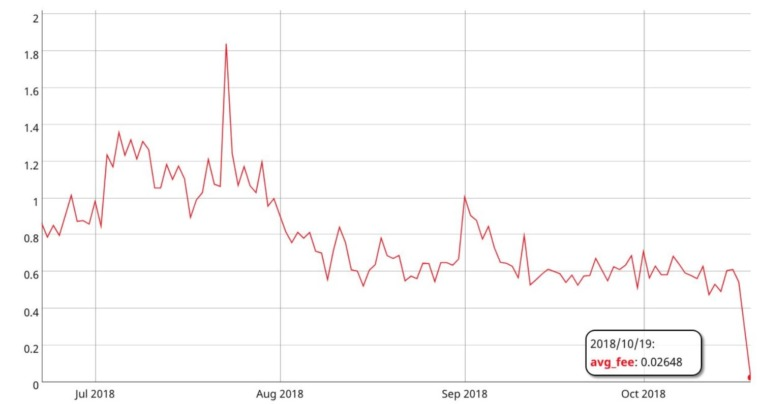
\includegraphics[width=0.8 \columnwidth,keepaspectratio]{Images/Monero/bulletproofs_2.jpg}
  \caption{July 2018 - October 2018.~\cite{bitinfocharts}}
  \label{fig:bulletproof_2}
\end{figure}
\vspace{0.3cm}
If we see this change in a broader time interval, the result is even more impressive:
\vspace{0.3cm}
\begin{figure}[H]
  \centering
  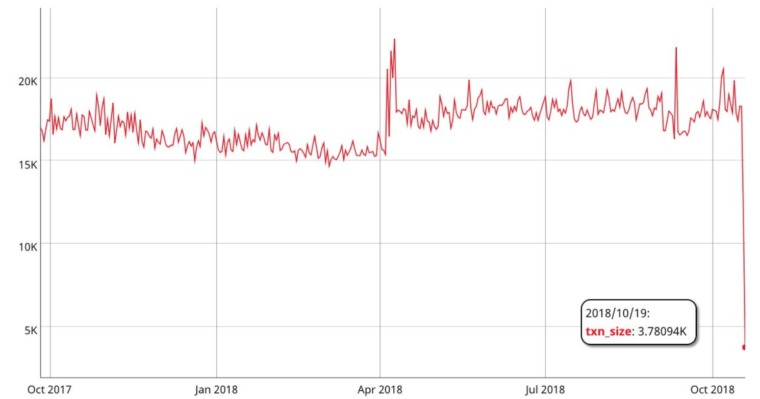
\includegraphics[width=0.8 \columnwidth,keepaspectratio]{Images/Monero/bulletproofs_1.jpg}
  \caption{July 2018 - October 2018.~\cite{bitinfocharts}}
  \label{fig:bulletproof_1}
\end{figure}
\pagebreak

There were predictions that the drop of fees might open the door to additional uses for XMR, the cryptocurrency that powers the Monero blockchain. Core developer \verb|hyc| said that the upgrade,
\begin{verbatim}
definitely [makes] the notion of micropayments more palatable again
\end{verbatim}
%%%%%%%%%%%%%%%%%%%%%%%%%%%%%%%%%%%%%%%%%%%%%%%%%%%%%%%%%%%%

\subsection{Kovri I2P Network} \label{sec:Kovri}
%\setlength{\intextsep}{0pt}
\begin{wrapfigure}[9]{L}{0.3\textwidth}
\centering

\includegraphics[height=0.28\textwidth]{Images/Kovri/kovri.jpg}
\end{wrapfigure}
Up to now, we have covered how Monero obfuscates information stored on the blockchain. Ring signatures obscure the sender. Stealth addresses prevent outside observers from knowing the receiving address. Finally, confidential transactions hide the amount of Monero transmitted. However, some personally identifiable information may be leaked at the network level when making a transaction. This privacy leak is addressed with Kovri~\cite{kovri}.

Kovri is a free, decentralized, anonymity technology based on I2P's open specifications~\cite{i2p}. Kovri uses both encryption and sophisticated routing techniques to create a private overlay-network across the Internet. This protected overlay allows users to hide their geographical location and IP address.

\subsubsection{Examples}
In the presentation of the project in the Gitlab page~\cite{git_kovri} some examples that Kovri's use protects a user's privacy are described. These examples will help the reader to understand the significance of Kovri's contribution to the anonymity level that Monero project aims to offer. Let's reproduce here these examples.

%\setlength{\intextsep}{0pt}
\begin{wrapfigure}[5]{R}{0.3\textwidth}
\centering

\includegraphics[height=0.15\textwidth]{Images/Kovri/trace.jpg}
\end{wrapfigure}
Suppose Alice wants to send Monero to Bob. Alice's wallet creates a transaction and then broadcasts it to the Monero network. The Monero network is made up of nodes that communicate with each other by directing messages using IP addresses. This means that it might be possible to geographically trace data as it travels over the open Internet, from start to finish and everywhere in between. Even though the sender's and recipient's wallet addresses - as well as the amount of Monero sent - remain private, Alice is taking a risk in broadcasting her transaction as some nodes may be logging IP addresses. An adversary with enough resources could attempt to associate transactions with IP addresses to determine from where transactions originate. This could potentially lead to an adversary not relaying her transactions to the rest of the network; or arriving at her front door!

Now let’s imagine a different scenario. Suppose Charlie wants to support the Monero network by running a full node at his home. After a few weeks, he receives a cease and desist letter from his Internet Service Provider claiming that running a node is a violation of the terms of service.

Or consider this, suppose Dave is an operator of a mining pool that donates a portion of block rewards to a political party or controversial cause. Other nodes could purposefully reject his solved blocks to express their disagreement with his political or social views.
\pagebreak

Alice, Bob, Charlie, and Dave all have at least one thing in common: their IP addresses were exposed. Users could try to hide IP addresses with the Tor~\cite{tor} or a VPN; however both of these strategies have serious weaknesses. The Tor network has "semi-trusted" Directory Authorities which give a handful of Tor node operators overreaching influence into network consensus. Network consensus ultimately determines who is allowed to relay traffic on the Tor network based on the views of the Directory Authorities. Furthermore, correlation attacks are easily possible with trusted VPNs, making it easy for large attackers to de-anonymize a user's traffic.

If Alice, Bob, Charlie, and Dave exclusively use Kovri to connect to the Monero network, no one will know their IP address, making passive surveillance impractical, while substantially improving Monero's censorship resistance.

\subsubsection{Technical Attributes}
%\setlength{\intextsep}{0pt}
\begin{wrapfigure}[7]{L}{0.2\textwidth}
\centering

\includegraphics[height=0.20\textwidth]{Images/Kovri/doll.png}
\end{wrapfigure}
Kovri tunnels traffic through the I2P network utilizing \emph{garlic encryption} and \emph{garlic routing}. The reader can find more about this technology in the I2P Network description~\cite{i2p}. Information travels within a private overlay-network by way of messages, which are encrypted in layers each time the message is passed along to peers in the network, similar to a Matryoshka doll.

For each inner doll there is a lock and public key to the next doll. Peers in the network are not able to read the contents of the message being relayed, so information sent from the sender to its destination (and vice-versa) are secured. The only information visible to peers is the instruction for sending messages to the next peer. To achieve greater privacy at a slight cost to performance, users are able to connect to several peers.

Essentially, Kovri covers an application's Internet traffic to make it anonymous within the network. Given this characteristic, Kovri is a great solution for anonymously communicating over IRC, email, or accessing hidden services. As Kovri is an open source project, the reader can find its full details in the project's Gitlab page~\cite{git_kovri}.
